%%%%%%%%%%%%%%%%%%%%%%%%%%%%%%%%%%%%%%%%%%%%%%%%%%%%%%%%%%%%%%%%%%%%%%%%%%%%%%%%
% Appendix-B.tex: Particle tracking
%%%%%%%%%%%%%%%%%%%%%%%%%%%%%%%%%%%%%%%%%%%%%%%%%%%%%%%%%%%%%%%%%%%%%%%%%%%%%%%%
% Outline:
% - Cross-correlation tracking method
% - Fourier transform based orientation analysis
%%%%%%%%%%%%%%%%%%%%%%%%%%%%%%%%%%%%%%%%%%%%%%%%%%%%%%%%%%%%%%%%%%%%%%%%%%%%%%%%
\chapter{Image Analysis Code}

\section{Code Vectorization}
\subsection{Vectorized Code for Spatial Correlation Function}
\begin{minted}
[
frame=lines,
framesep=2mm,
baselinestretch=1.1,
linenos,
]
{python}

def corrS(X, Y, U, V):
    row, col = X.shape
    vsqrt = (U ** 2 + V ** 2) ** 0.5
    U = U - U.mean()
    V = V - V.mean()
    Ax = U / vsqrt
    Ay = V / vsqrt
    CA = np.ones(X.shape)
    CV = np.ones(X.shape)
    for xin in range(0, col):
        for yin in range(0, row):
            if xin != 0 or yin != 0:
                CA[yin, xin] = (Ax[0:row-yin, 0:col-xin] * Ax[yin:row, xin:col] + Ay[0:row-yin, 0:col-xin] * Ay[yin:row, xin:col]).mean()
                CV[yin, xin] = (U[0:row-yin, 0:col-xin] * U[yin:row, xin:col] + V[0:row-yin, 0:col-xin] * V[yin:row, xin:col]).mean() / (U.std()**2+V.std()**2)
    return CA, CV
\end{minted}

\subsection{Non-vectorized Code for Spatial Correlation Function}
\begin{minted}
[
frame=lines,
framesep=2mm,
baselinestretch=1.1,
linenos,
]
{python}
def corrS(X, Y, U, V):
    row, col = X.shape
    vsq = 0
    CA = np.zeros((row, col))
    CV = np.zeros((row, col))
    for i in range(0, row):
        for j in  range(0, col):
            vsq += U[i, j]**2 + V[i, j]**2
    for xin in range(0, col):
        for yin in range(0, row):
            count = 0
            CAt = 0
            CVt = 0
            for i in range(0, col-xin):
                for j in range(0, row-yin):
                    ua = U[j, i]
                    va = V[j, i]
                    ub = U[j+yin, i+xin]
                    vb = V[j+yin, i+xin]
                    CAt += (ua*ub+va*vb)/((ua**2+va**2)*(ub**2+vb**2))**.5
                    CVt += ua*ub + va*vb
                    count += 1
            CA[yin, xin] = CAt / count
            CV[yin, xin] = CVt / vsq
    return CA, CV
\end{minted}


\begin{figure}[!ht]
	\begin{center}
	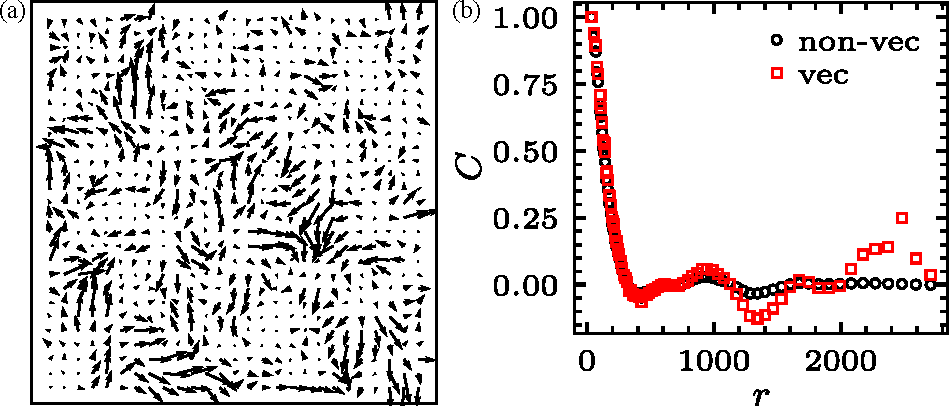
\includegraphics[width=5.5in]{Figs/A-2/vectorization.pdf}
	%select pdftexify command to run jpg or pdf files
	\end{center}
	\caption[Compare the performance of vectorized and non-vectorized code]
	{
	\textbf{Compare the performance of vectorized and non-vectorized code.}
  (a) Sample velocity field.
  (b) Velocity correlation functions obtained from the vectorized and non-vectorized code.
	}
	\label{fig:vectorization-performance}
\end{figure}


\subsection{Performance Comparison}
We notice that the vectorized code has two less nested \texttt{for} loops compared to the non-vectorized code. As a result, the vectorized one runs much faster for the same task. To quantify this performance difference, we perform the spatial correlation function calculation using both code on the same velocity field, shown in Fig.~\ref{fig:vectorization-performance}a. The times taken for the two functions are:
\begin{itemize}
  \item \texttt{Vectorized code: 0.84 s}
  \item \texttt{Non-vectorized code: 52.06 s}
\end{itemize}
The result is shown in Fig.~\ref{fig:vectorization-performance}b. Although in the large $r$ regime, two methods show descrepancies, in the meaningful small $r$ regime, two methods give exactly the same results.


\section{Energy Spectrum Calculation}
The following code is used for calculating the energy spectra in Chap.~\ref{giant-number-fluctuations-in-3-dimensional-space}.

\begin{minted}
[
frame=lines,
framesep=2mm,
baselinestretch=1.1,
linenos,
]
{python}
def compute_energy_density(pivData, d=25*0.33, MPP=0.33):
    """
    Compute kinetic energy density in k space from piv data. The unit of the return value is [velocity] * [length],
    where [velocity] is the unit of pivData, and [length] is the unit of sample_spacing parameter.
    Note, the default value of sampling_spacing does not have any significance. It is just the most convenient value for my first application,
    and should be set with caution when a different magnification and PIV are used.

    Args:
    pivData -- piv data
    d -- sample spacing
    MPP -- microns per pixel

    Returns:
    E -- kinetic energy field in k space
    """

    row = len(pivData.y.drop_duplicates())
    col = len(pivData.x.drop_duplicates())
    U = np.array(pivData.u).reshape((row, col)) * MPP
    V = np.array(pivData.v).reshape((row, col)) * MPP

    u_fft = np.fft.fft2(U) * d * d
    v_fft = np.fft.fft2(V) * d * d

    E = (u_fft * u_fft.conjugate() + v_fft * v_fft.conjugate()) / 2

    return E

def compute_wavenumber_field(shape, d):
    """
    Compute the wave number field Kx and Ky, and magnitude field k.
    Note that this function works for even higher dimensional shape.

    Args:
    shape -- shape of the velocity field and velocity fft field, tuple
    d -- sample spacing. This is the distance between adjacent samples, for example, velocities in PIV.
        The resulting frequency space has the unit which is inverse of the unit of d. The preferred unit of d is um.

    Returns:
    k -- wavenumber magnitude field
    K -- wavenumber fields in given dimensions
    """

    for num, length in enumerate(shape):
        kx = np.fft.fftfreq(length, d=d)
        if num == 0:
            k = (kx,)
        else:
            k += (kx,)

    K = np.meshgrid(*k, indexing='ij')

    for num, k1 in enumerate(K):
        if num == 0:
            ksq = k1 ** 2
        else:
            ksq += k1 ** 2

    k_mag = ksq ** 0.5 * 2 * np.pi

    return k_mag, K

def energy_spectrum(pivData, d=25*0.33):
    """
    Compute energy spectrum (E vs k) from pivData.

    Args:
    pivData -- piv data
    d -- sample spacing. This is the distance between adjacent samples, for example, velocities in PIV.
        The resulting frequency space has the unit which is inverse of the unit of d. The default unit of d is um.

    Returns:
    es -- energy spectrum, DataFrame (k, E)
    """

    row = len(pivData.y.drop_duplicates())
    col = len(pivData.x.drop_duplicates())

    E = compute_energy_density(pivData, d) / (row * d * col * d)
    k, K = compute_wavenumber_field(E.shape, d)

    ind = np.argsort(k.flatten())
    k_plot = k.flatten()[ind]
    E_plot = E.real.flatten()[ind]

    es = pd.DataFrame(data={'k': k_plot, 'E': E_plot})

    return es
\end{minted}

\section{Cross-Correlation Based Particle Detecting Method}
\label{cross-correlation-tracking-method}
This is designed for tracking colloidal chains. We show here the basic working principle and the code here. The advantage of this method is that it does not require the feature to be very bright or dark, like traditional particle detecting methods. As long as the features share similar characteristics, i.e. spatial patterns, this method can work well.

\subsection{Working principle}
From raw images, we crop out a single feature which we are looking for as a target mask, as shown in Fig.~\ref{fig:corr-track}a inset. Then, we do a 2D correlation between the target mask and an image (Fig.~\ref{fig:corr-track}a). The resulting correlation map is shown in Fig.~\ref{fig:corr-track}b, where bright pixels stand for high correlation and dark pixels stand for low correlation. The last step is to look for the pixel intensity peaks in the correlation map, as in traditional particle detecting methods.

\begin{figure}[h]
	\begin{center}
	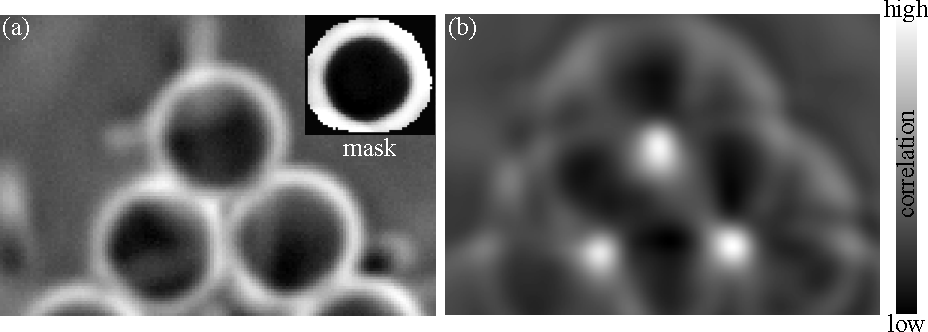
\includegraphics[width=5.5in]{Figs/A-2/corrTrack.pdf}
	%select pdftexify command to run jpg or pdf files
	\end{center}
	\caption[Cross-correlation based particle detecting method]
	{
	\textbf{Cross-correlation based particle detecting method.}
  (a) A sample image of colloidal particles. Inset: a mask produced by cropping the raw image and binarize.
  (b) The cross-correlation map.
	}
	\label{fig:corr-track}
\end{figure}

\subsection{Code}
\begin{minted}[frame=lines,framesep=2mm,baselinestretch=1.1,linenos]{python}
import numpy as np
from scipy.signal import medfilt2d, convolve2d, fftconvolve
from math import exp

def normxcorr2(template, image, mode="full"):
    if np.ndim(template) > np.ndim(image) or \
            len([i for i in range(np.ndim(template)) if template.shape[i] > image.shape[i]]) > 0:
        print("normxcorr2: TEMPLATE larger than IMG. Arguments may be swapped.")
    template = template - np.mean(template)
    image = image - np.mean(image)
    a1 = np.ones(template.shape)
    ar = np.flipud(np.fliplr(template))
    out = fftconvolve(image, ar.conj(), mode=mode)
    image = fftconvolve(np.square(image), a1, mode=mode) - \
            np.square(fftconvolve(image, a1, mode=mode)) / (np.prod(template.shape))
    image[np.where(image < 0)] = 0
    template = np.sum(np.square(template))
    out = out / np.sqrt(image * template)
    out[np.where(np.logical_not(np.isfinite(out)))] = 0
    return -out

def matlab_style_gauss2D(shape=(3,3),sigma=0.5):
    m,n = [(ss-1.)/2. for ss in shape]
    y,x = np.ogrid[-m:m+1,-n:n+1]
    h = np.exp( -(x*x + y*y) / (2.*sigma*sigma) )
    h[ h < np.finfo(h.dtype).eps*h.max() ] = 0
    sumh = h.sum()
    if sumh != 0:
        h /= sumh
    return h

def FastPeakFind(data):
    if str(data.dtype) != 'float32':
        data = data.astype('float32')
    mf = medfilt2d(data, kernel_size=3)
    mf = mf.astype('float32')
    thres = max(min(np.amax(mf,axis=0)), min(np.amax(mf,axis=1)))
    filt = matlab_style_gauss2D()
    conv = convolve2d(mf, filt, mode='same')
    w_idx = conv > thres
    bw = conv.copy()
    bw[w_idx] = 1
    bw[~w_idx] = 0
    thresholded = np.multiply(bw, conv)
    edg = 3
    shape = data.shape
    idx = np.nonzero(thresholded[edg-1: shape[0]-edg-1, edg-1: shape[1]-edg-1])
    idx = np.transpose(idx)
    cent = []
    for xy in idx:
        x = xy[0]
        y = xy[1]
        if thresholded[x, y] >= thresholded[x-1, y-1] and \
            thresholded[x, y] > thresholded[x-1, y] and \
            thresholded[x, y] >= thresholded[x-1, y+1] and \
            thresholded[x, y] > thresholded[x, y-1] and \
            thresholded[x, y] > thresholded[x, y+1] and \
            thresholded[x, y] >= thresholded[x+1, y-1] and \
            thresholded[x, y] > thresholded[x+1, y] and \
            thresholded[x, y] >= thresholded[x+1, y+1]:
            cent.append(xy)
    cent = np.asarray(cent).transpose()
    return cent

def maxk(array, num_max):
    array = np.asarray(array)
    length = array.size
    array = array.reshape((1, length))
    idx = np.argsort(array)
    idx2 = np.flip(idx)
    return idx2[0, 0:num_max]

def gauss1(x,a,x0,sigma):
    return a*exp(-(x-x0)**2/(2*sigma**2))

def track_spheres(img, mask, num_particles):
    def gauss1(x,a,x0,sigma):
        return a*exp(-(x-x0)**2/(2*sigma**2))
    corr = normxcorr2(mask, img, mode='same')
    cent = FastPeakFind(corr)
    peaks = corr[cent[0], cent[1]]
    ind = maxk(peaks, num_particles)
    max_coor_tmp = cent[:, ind]
    max_coor = max_coor_tmp.astype('float32')
    pk_value = peaks[ind]
    for num in range(0, num_particles):
        x = max_coor_tmp[0, num]
        y = max_coor_tmp[1, num]
        fitx1 = np.asarray(range(x-7, x+8))
        fity1 = np.asarray(corr[range(x-7, x+8), y])
        popt, pcov = curve_fit(gauss1, fitx1, fity1, p0=[1, x, 3])
        max_coor[0, num] = popt[1]
        fitx2 = np.asarray(range(y-7, y+8))
        fity2 = np.asarray(corr[x, range(y-7, y+8)])
        popt,pcov = curve_fit(gauss1, fitx2, fity2, p0=[1, y, 3])
        max_coor[1, num] = popt[1]
    return max_coor, pk_value
\end{minted}


\section{Fourier Transform Based Orientation Analysis}
\label{fourier-transform-based-orientation-analysis}

\section{Density Fluctuation Calculation}
